\documentclass{standalone}
\usepackage{tikz}
\usepackage{pgfplots}
\begin{document}


    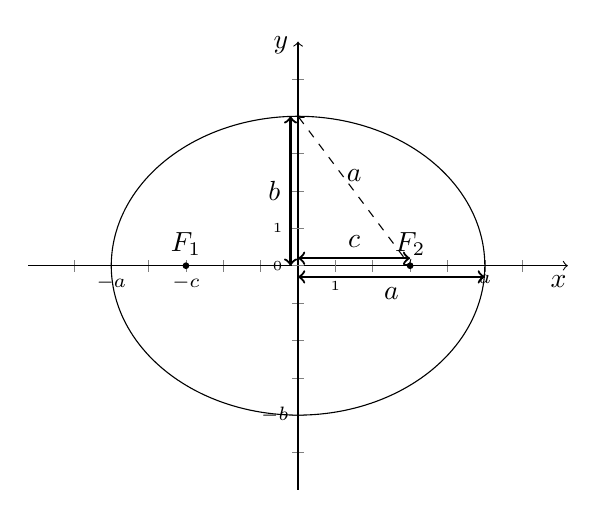
\begin{tikzpicture}[scale = 1]
\begin{axis}[
    xmin=-7, xmax=7,
    ymin=-6, ymax=6,
    %grid=both,
    axis lines=middle,
    %minor tick num=1,
    axis line style={->},
    ticklabel style={font=\tiny},
    axis equal,
    xticklabels=\empty,
    yticklabels=\empty,
    xlabel={$x$},
    ylabel={$y$},
    extra x ticks={1},
    extra y ticks={0,1},
    xtick={-6,-5, -4, -3,-2,-1,0,1,2,3,4,5,6},
    ytick={-5, -4, -3,-2,-1,0,1,2,3,4,5},
    xlabel style={at={(axis description cs:0.95,0.5)}, anchor=north west},
    ylabel style={at={(axis description cs:0.5,0.95)}, anchor=south east}
]

% Ellipse
%\draw (axis cs:0,0) ellipse [x radius=5, y radius=4];
\addplot [domain=0:360, samples=200] 
  ({5*cos(x)}, {4*sin(x)});

% Focus F2
\filldraw (axis cs:3,0) circle (1pt);
\node[above ] at (axis cs:3,0) {$F_2$};

% Focus F1
\filldraw (axis cs:-3,0) circle (1pt);
\node[above ] at (axis cs:-3,0) {$F_1$};

% Focus S1
%\filldraw (axis cs:-5,0) circle (1pt);
\node[below  ] at (axis cs:-5,0) {\scriptsize$-a$};


% Focus S2
%\filldraw (axis cs:5,0) circle (1pt);
%\node[below  ] at (axis cs:3,0) {\scriptsize$c$};

% Focus S1
%\filldraw (axis cs:-5,0) circle (1pt);
\node[below  ] at (axis cs:-3,0) {\scriptsize$-c$};


% Focus S2
%\filldraw (axis cs:5,0) circle (1pt);
\node[below] at (axis cs:5,0) {\scriptsize$a$};

% Focus S3
%\filldraw (axis cs:0, 3) circle (1pt);
%\node[ left ] at (axis cs:0, 4) {\scriptsize$b$};

% Focus S4
%\filldraw (axis cs:0, -3) circle (1pt);
\node[ left ] at (axis cs:0, -4) {\scriptsize$-b$};

\draw[<->, dashed] (axis cs:0,4) -- (axis cs:3,0) node[midway, above] {$a$};

% Draw a double-headed arrow
\draw[<->, thick] 
  (axis cs:0,0.2) -- (axis cs:3,0.2) 
  node[midway, above] {$c$};
  
\draw[<->, thick] 
  (axis cs:0,-0.3) -- (axis cs:5,-0.3) 
  node[midway, below] {$a$};
  \draw[<->, thick] 
  (axis cs:-0.2,0) -- (axis cs:-0.2,4) 
  node[midway, left] {$b$};
\end{axis}
\end{tikzpicture}

\end{document}